%%
%% 2019 07 04 Ph. G. Freimann
%%

\section{Ähnlichkeit}\index{Ähnlichkeit}
\sectuntertitel{Treffen sich zwei Parallele.}
%%%%%%%%%%%%%%%%%%%%%%%%%%%%%%%%%%%%%%%%%%%%%%%%%%%%%%%%%%%%%%%%%%%%%%%%%%%%%%%%%
\theorieTALSGeom{63}{1.5}\\
\theorieTALSGeom{69}{1.5.2 (ähnliche Figuren)}\\
\theorieTALSGeom{72}{1.5.3 (ähnliche Dreiecke)}\\
\theorieTALSGeom{81}{1.5.4 (Ähnlichkeit am Kreis)}

\subsection*{Lernziele}

\begin{itemize}
\item Translation
\item Drehung
\item Streckung
\item Spiegelung
%%\item Scherung (Lernziel ???)
\end{itemize}

\raisebox{-2cm}{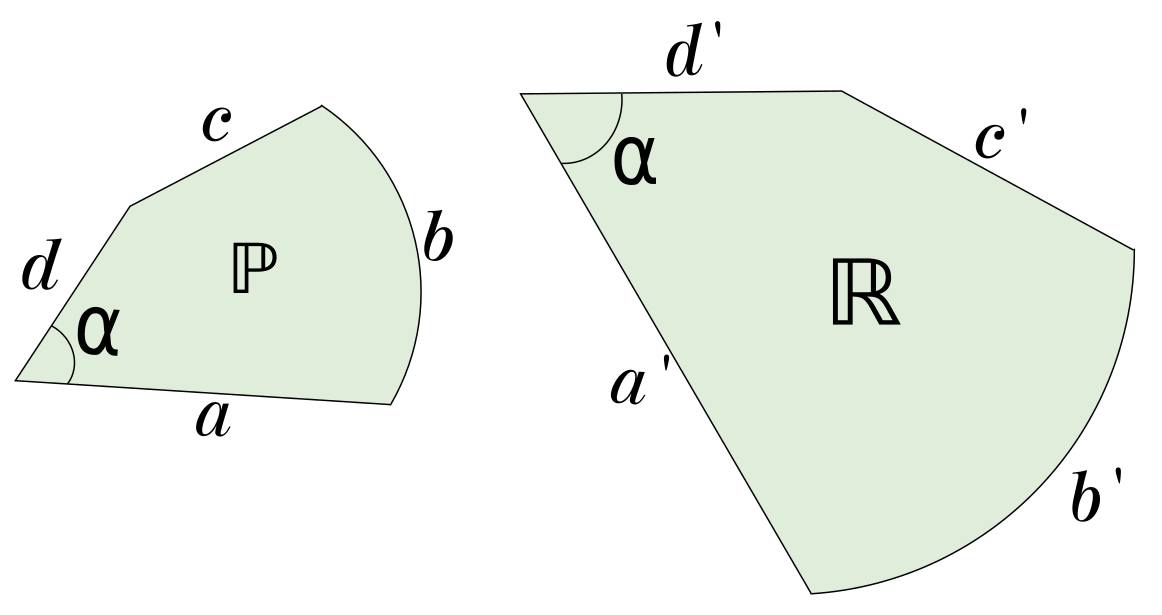
\includegraphics[width=11cm]{tals/plani/img/aehnlichkeit.png}}

In ähnlichen Figuren sind die entsprechenden Winkel gleich.

\begin{definition}{Ähnliche Figuren}{}
Sind zwei Figuren ähnlich, so existiert ein \textbf{Streckungsfaktor}
$k$, der die Strecken der einen Figur auf die andere «abbildet»:
$$a' = k\cdot{}a; b' = k\cdot{}b; c' = k\cdot{} c; ...$$
\end{definition}

Daraus ergibt sich durch Division:
\begin{gesetz}{Streckungsfaktor}{}
  $$k = \frac{a'}{a} = \frac{b'}{b} = \frac{c'}{c} = ...$$
\end{gesetz}

\newpage


Für die Flächen gilt jedoch

\begin{gesetz}{Flächen ähnlicher Figuren}{}
$$\frac{|\mathbb{A}|}{|\mathbb{A'}|} = k^2$$
\end{gesetz}

\TALSGeomAadB{64ff (zentrische Streckung)}{257. 264. 271. (berechnen)}
\TALSGeomAadB{69ff (ähnliche Figuren)}{279. 283. 286. 290.}
\TALSGeomAadB{73ff (ähnliche Dreiecke)}{306. 309. 319.}
\TALSGeomAadB{81ff (Ähnlichkeit am Kreis)}{338. 340. 341. 342.}

\GESOAadB{???}{???}

